\section{实验要求与实验目的}

\subsection{实验要求}
本实验要求利用 AT89C51 单片机和两片 SN74HC573 数据锁存器完成 LED 数码管动态显示。由于 AT89C51 的 P0 口直接驱动能力和端口数量有限，本实验把 P0.0--P0.7 作为复用数据总线，分别送入两片 SN74HC573：一片锁存段码，另一片锁存位码。P2.6 用于控制段码锁存器的 LE 端，P2.7 用于控制位选锁存器的 LE 端。系统复位后，在 8 位共阴极 LED 数码管上动态显示 ``HELLO-88''。

完整电路需要包含单片机供电、复位电路、晶振电路、P0 口上拉电阻、两片 SN74HC573 锁存电路和 8 位共阴极 LED 数码管显示电路，并完成程序编写与 Proteus 仿真调试。

\subsection{实验目的}
\begin{enumerate}
  \item 了解八段共阴极 LED 数码管的段选、位选和动态扫描显示原理。
  \item 掌握利用 AT89C51 并行 I/O 口驱动 LED 数码管的方法。
  \item 掌握 SN74HC573 锁存器扩展 P0 口、分时输出段码和位码的接口设计方法。
  \item 熟悉 ASEM-51 汇编程序结构、段码表查表和显示缓冲区设计。
\end{enumerate}

\subsection{总体设计思路}
系统以 AT89C51 为控制核心，P0 口作为 8 位复用数据总线。输出段码时，程序把段码送到 P0，再通过 P2.6 给段码锁存器一个锁存脉冲；输出位码时，程序把位选码送到 P0，再通过 P2.7 给位选锁存器一个锁存脉冲。由于两片锁存器的输出会保持最近一次锁存的数据，单片机只需按位快速刷新，便可以利用视觉暂留让 8 位数码管看起来同时点亮。

\begin{figure}[H]
\centering
\resizebox{0.95\textwidth}{!}{%
\begin{tikzpicture}[
  node distance=10mm and 14mm,
  block/.style={rectangle,rounded corners,draw=themecolor,fill=blue!3,minimum width=3.7cm,minimum height=9mm,align=center},
  io/.style={trapezium,trapezium left angle=75,trapezium right angle=105,draw=accentgreen,fill=green!8,minimum width=3.8cm,minimum height=9mm,align=center},
  note/.style={rectangle,rounded corners,draw=softline,fill=white,minimum width=5.0cm,minimum height=7mm,align=center,font=\small},
  line/.style={-Latex,thick,draw=themecolor}
]
  \node[block] (mcu) {AT89C51\\P0 数据总线};
  \node[block,right=of mcu,yshift=8mm] (seg573) {SN74HC573\\段码锁存};
  \node[block,right=of mcu,yshift=-8mm] (bit573) {SN74HC573\\位码锁存};
  \node[io,right=18mm of seg573,yshift=-8mm] (led) {8 位共阴极\\LED 数码管};

  \draw[line] (mcu) -- node[above,font=\small] {P0.0--P0.7} (seg573);
  \draw[line] (mcu) -- node[below,font=\small] {P0.0--P0.7} (bit573);
  \draw[line] (seg573) -- node[above,font=\small] {A--DP} (led);
  \draw[line] (bit573) -- node[below,font=\small] {1--8 位选} (led);
  \node[note,below=10mm of mcu] {P2.6：段码锁存器 LE\\P2.7：位选锁存器 LE};
\end{tikzpicture}}
\caption{实验四 LED 数码管显示系统结构}
\end{figure}

\section{硬件电路设计}

\subsection{单片机最小系统}
AT89C51 采用 +5V 供电。XTAL1 与 XTAL2 外接晶振和两个 30pF 电容，构成单片机时钟电路。EA 引脚接高电平，使单片机从片内程序存储器取指。RST 引脚连接复位网络，上电时由电容充电形成复位脉冲，按下复位按钮时也可以使程序重新从 0000H 开始执行。

\begin{figure}[H]
  \centering
  \begin{subfigure}{0.58\textwidth}
    \centering
    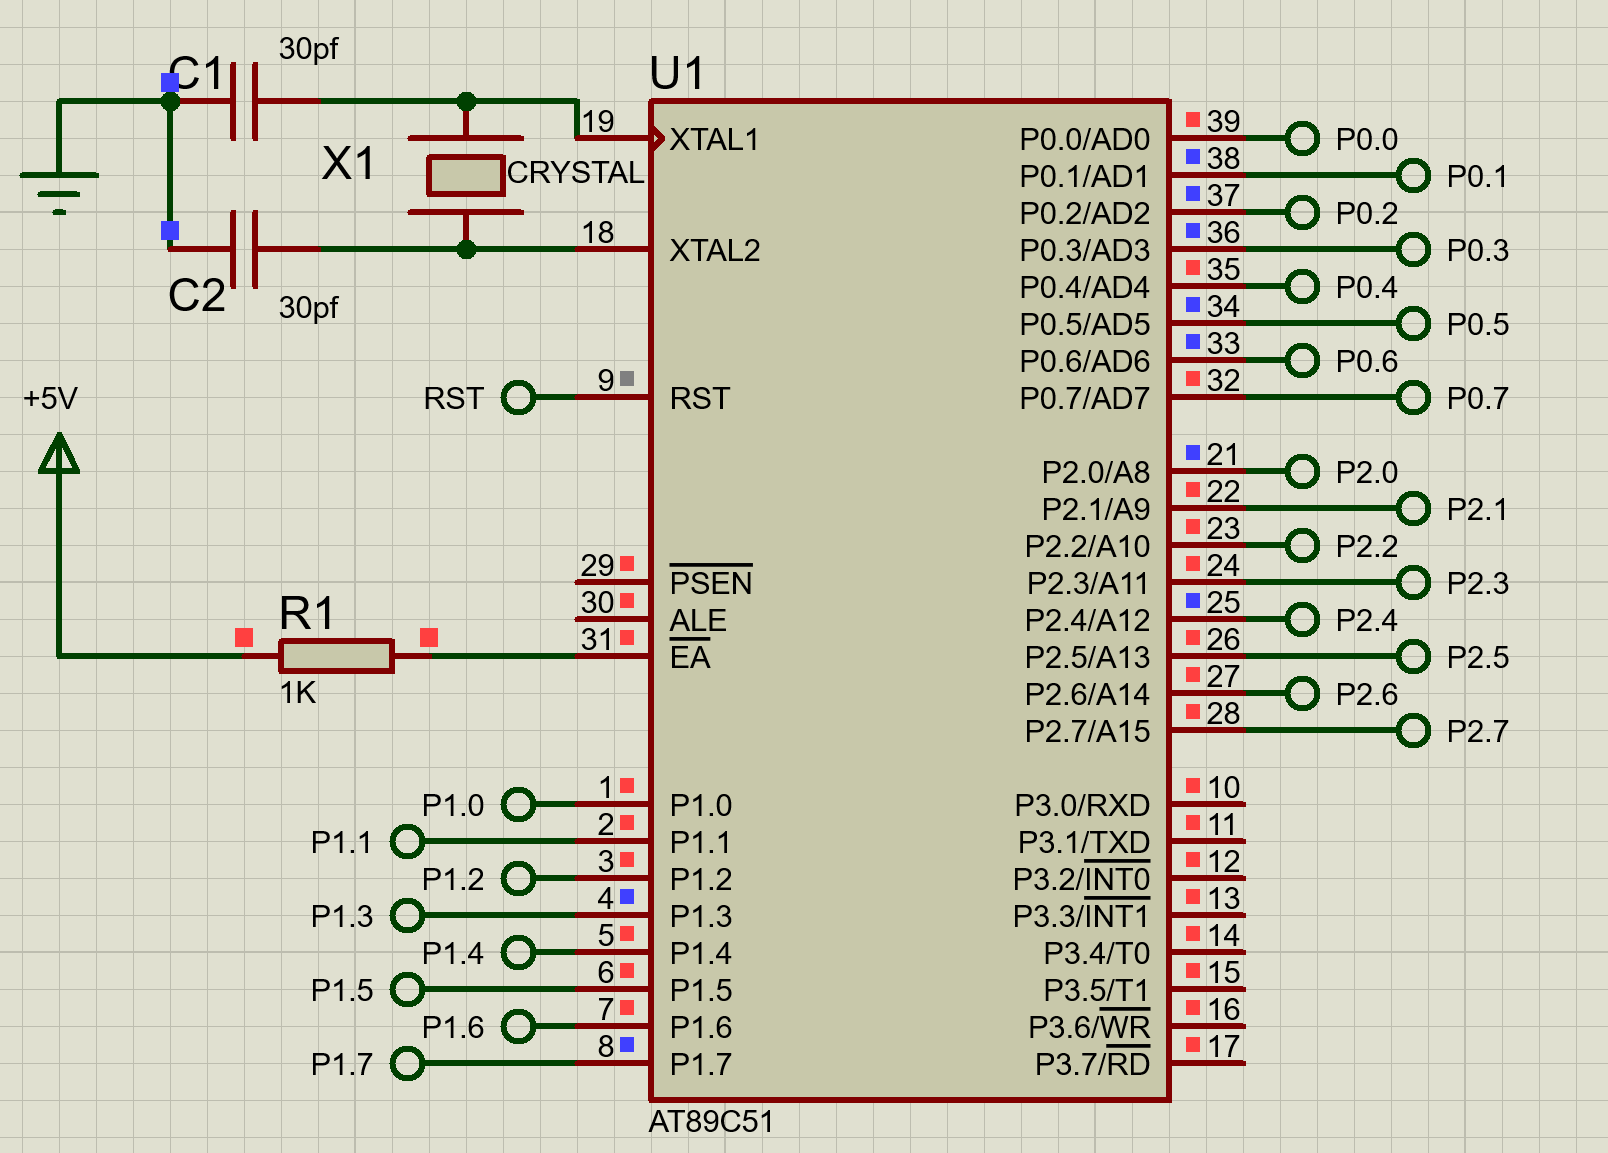
\includegraphics[width=\textwidth]{images/power.png}
    \caption{AT89C51 供电与晶振电路}
  \end{subfigure}
  \hfill
  \begin{subfigure}{0.34\textwidth}
    \centering
    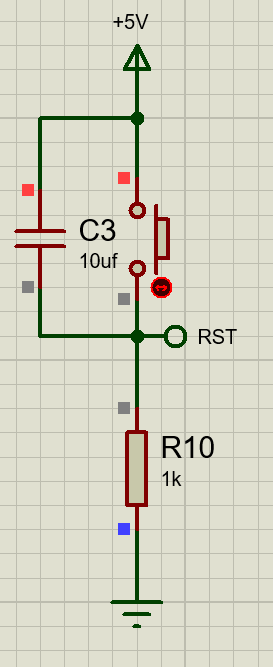
\includegraphics[width=\textwidth]{images/rst.png}
    \caption{复位电路}
  \end{subfigure}
  \caption{单片机基础外围电路}
\end{figure}

\subsection{SN74HC573 扩展 P0 口}
AT89C51 的 P0 口为漏极开路结构，作为普通 I/O 使用时需要外接上拉电阻。本实验中 P0.0--P0.7 同时连接两片 SN74HC573 的 D0--D7 输入端，P0 上的数据由 P2.6、P2.7 分别锁存到不同的输出通道。两片 SN74HC573 的 OE 接地，使输出始终允许。

段码锁存器的 Q0--Q7 连接数码管 A、B、C、D、E、F、G、DP 段；位码锁存器的 Q0--Q7 连接数码管第 1--8 位公共端。程序先关闭所有位选，再送段码和位码，可以减小动态扫描时的重影。

\subsection{共阴极 LED 动态显示}
共阴极数码管的段信号为高电平有效，位选公共端为低电平有效。程序中的位码从 \texttt{0FEH} 开始，表示只有最低位为 0，即选通第 1 位；随后通过 \texttt{RL A} 左移，依次得到 \texttt{0FDH}、\texttt{0FBH}、\texttt{0F7H} 等位选码，从左到右扫描 8 位数码管。

\begin{table}[H]
  \centering
  \caption{主要端口分配}
  \renewcommand{\arraystretch}{1.35}
  \begin{tabular}{p{0.22\textwidth}p{0.34\textwidth}p{0.34\textwidth}}
    \toprule
    单片机端口 & 连接对象 & 功能说明 \\
    \midrule
    P0.0--P0.7 & 两片 SN74HC573 的 D0--D7 & 复用输出段码和位码 \\
    P2.6 & 段码锁存器 LE & 锁存 A--DP 段码 \\
    P2.7 & 位码锁存器 LE & 锁存第 1--8 位位选码 \\
    EA & +5V & 片内程序存储器有效 \\
    RST & 复位网络 & 上电和按键复位 \\
    XTAL1/XTAL2 & 晶振与 30pF 电容 & 提供单片机工作时钟 \\
    \bottomrule
  \end{tabular}
\end{table}

\subsection{Proteus 仿真电路}
图 \ref{fig:key} 为实验四 Proteus 仿真关键电路。图中 P0 口通过电阻排上拉后连接两片 74HC573，两片锁存器分别连接数码管的段线和位选线。运行程序后，数码管能够动态显示 ``HELLO-88''，其中字母 O 由七段数码管中的数字 0 近似表示。

\begin{figure}[H]
  \centering
  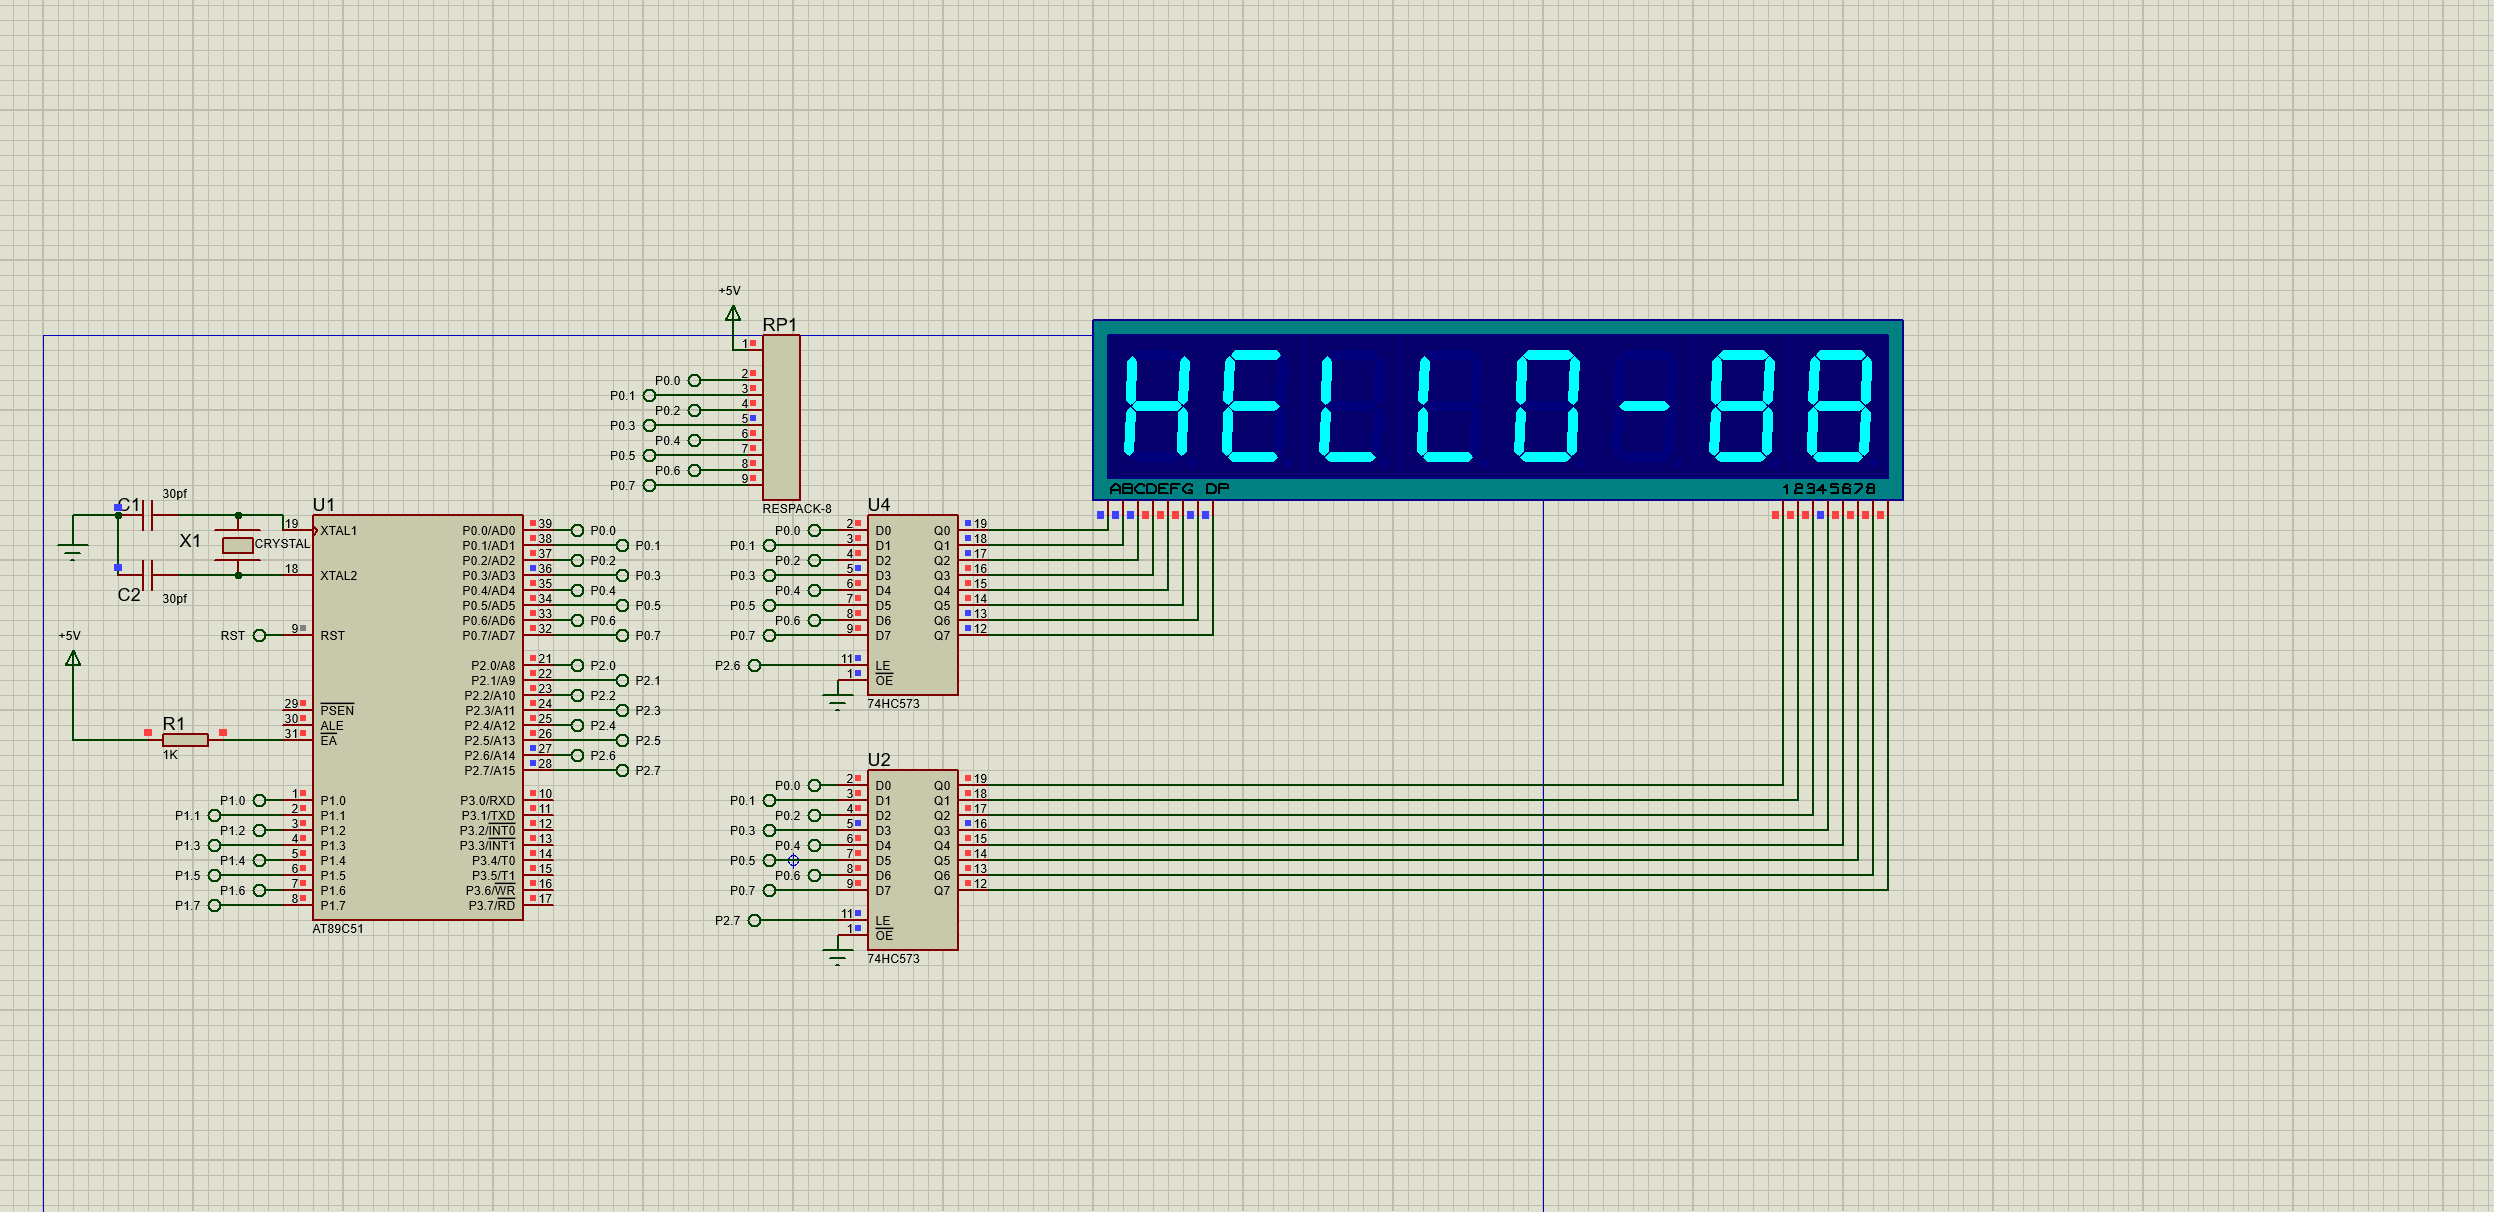
\includegraphics[width=0.95\textwidth]{images/experiment4_key.png}
  \caption{实验四 LED 数码管显示关键仿真图}
  \label{fig:key}
\end{figure}

\section{软件设计}

\subsection{程序设计思路}
程序首先初始化堆栈指针和显示缓冲区。显示缓冲区从内部 RAM 的 50H 开始，共 8 个单元，依次保存 H、E、L、L、O、-、8、8 的段码索引。主循环不断调用显示扫描逻辑，每次从 50H 开始读取显示缓冲单元，查段码表得到真实段码，然后送入段码锁存器；再把当前位选码送入位码锁存器。每显示一位后进行短延时，再扫描下一位。

\begin{figure}[H]
\centering
\begin{tikzpicture}[
  node distance=8mm,
  proc/.style={rectangle,rounded corners,draw=themecolor,fill=blue!3,minimum width=7.2cm,minimum height=8mm,align=center},
  term/.style={ellipse,draw=accentgreen,fill=green!8,minimum width=4.2cm,minimum height=8mm,align=center},
  line/.style={-Latex,thick,draw=themecolor}
]
  \node[term] (start) {开始};
  \node[proc,below=of start] (init) {初始化 SP、显示缓冲区和锁存控制位};
  \node[proc,below=of init] (disp) {执行动态显示扫描};
  \node[proc,below=of disp] (loop) {返回继续刷新};

  \draw[line] (start) -- (init);
  \draw[line] (init) -- (disp);
  \draw[line] (disp) -- (loop);
  \draw[line] (loop.east) -- ++(1,0) |- (disp.east);
\end{tikzpicture}
\caption{主程序流程图}
\end{figure}

\subsection{显示扫描流程}
显示扫描部分的核心是“先消隐、再送段码、再送位码”。这样可以避免上一位的位选仍然有效时段码发生变化，从而减小重影。扫描码初值为 \texttt{0FEH}，每轮扫描后左移一位。当最高位已经移出扫描范围时，程序关闭段码和位码后重新开始下一轮扫描。

\begin{figure}[H]
\centering
\resizebox{0.68\textwidth}{!}{%
\begin{tikzpicture}[
  node distance=5mm,
  proc/.style={rectangle,rounded corners,draw=themecolor,fill=blue!3,minimum width=7.2cm,minimum height=7mm,align=center},
  judge/.style={diamond,aspect=2.2,draw=accentyellow,fill=yellow!10,minimum width=4.0cm,minimum height=8mm,align=center},
  line/.style={-Latex,thick,draw=themecolor}
]
  \node[proc] (s1) {设定显示缓冲区首地址 R0=50H};
  \node[proc,below=of s1] (s2) {设定扫描码初值 30H=0FEH};
  \node[proc,below=of s2] (s3) {清位控码，关闭所有位选};
  \node[proc,below=of s3] (s4) {读取显示缓冲区，查段码表};
  \node[proc,below=of s4] (s5) {送段码到 P0，P2.6 锁存};
  \node[proc,below=of s5] (s6) {送位码到 P0，P2.7 锁存};
  \node[proc,below=of s6] (s7) {延时，保持当前位显示};
  \node[proc,below=of s7] (s8) {显示缓冲区地址加 1，扫描码左移};
  \node[judge,below=of s8] (s9) {扫描码是否到头};
  \node[proc,below=of s9] (s10) {清段码、清位码，返回下一轮};

  \draw[line] (s1) -- (s2);
  \draw[line] (s2) -- (s3);
  \draw[line] (s3) -- (s4);
  \draw[line] (s4) -- (s5);
  \draw[line] (s5) -- (s6);
  \draw[line] (s6) -- (s7);
  \draw[line] (s7) -- (s8);
  \draw[line] (s8) -- (s9);
  \draw[line] (s9) -- node[right,font=\small] {是} (s10);
  \draw[line] (s9.east) -- ++(1.1,0) |- node[right,font=\small,pos=0.25] {否} (s3.east);
\end{tikzpicture}}
\caption{显示子程序流程图}
\end{figure}

\subsection{显示字符与段码表}
七段数码管不能像点阵屏一样显示标准字母，因此本实验使用可识别的近似字符。程序中显示缓冲区保存的是段码表索引，实际显示时再通过 \texttt{MOVC A,@A+DPTR} 查表得到段码。

\begin{table}[H]
  \centering
  \caption{HELLO-88 显示缓冲区与段码}
  \renewcommand{\arraystretch}{1.35}
  \begin{tabular}{cccc}
    \toprule
    显示位置 & 缓冲区地址 & 缓冲区索引 & 查表后段码 \\
    \midrule
    1 & 50H & 11H & 76H，显示 H \\
    2 & 51H & 0EH & 79H，显示 E \\
    3 & 52H & 12H & 38H，显示 L \\
    4 & 53H & 12H & 38H，显示 L \\
    5 & 54H & 00H & 3FH，显示 0 近似 O \\
    6 & 55H & 13H & 40H，显示 - \\
    7 & 56H & 08H & 7FH，显示 8 \\
    8 & 57H & 08H & 7FH，显示 8 \\
    \bottomrule
  \end{tabular}
\end{table}

\subsection{完整源程序}
\lstset{style=a51style}
\lstinputlisting[caption={04\_lcd.A51 完整源程序}]{code/04_lcd.A51}

\section{仿真调试与结果分析}

\subsection{调试步骤}
\begin{enumerate}
  \item 检查 AT89C51 的 +5V 电源、EA、晶振和复位电路，确认程序能够从复位地址启动。
  \item 检查 P0 口是否接上拉电阻排，避免 P0 开漏输出导致高电平异常。
  \item 检查两片 SN74HC573 的 D0--D7 是否都接到 P0.0--P0.7，OE 是否接地。
  \item 检查 P2.6 是否接段码锁存器 LE，P2.7 是否接位码锁存器 LE。
  \item 单独测试第一位显示 0，确认段线顺序和第一位位选正确。
  \item 加载完整程序，观察 8 位数码管是否稳定显示 ``HELLO-88''。
\end{enumerate}

\subsection{仿真现象}
在 Proteus 中运行程序后，8 位共阴极数码管动态显示 ``HELLO-88''。由于七段数码管的显示能力有限，字母 O 使用数字 0 的段码近似显示，因此实际视觉效果为 ``HELL0-88''。H、E、L、-、8 等字符均通过段码表实现，显示稳定，说明 P0 扩展、锁存控制和动态扫描逻辑均能正常工作。

\subsection{问题分析}
本实验调试中最容易出现的问题是段码和位码接线顺序不一致。若段码锁存器 Q0--Q7 没有按 A、B、C、D、E、F、G、DP 顺序连接，字符会显示成错误形状；若位码锁存器 Q0--Q7 与第 1--8 位顺序不一致，则字符顺序会颠倒或错位。此外，P0 口必须接上拉电阻，否则高电平输出不可靠。通过固定段码 \texttt{3FH}、固定位码 \texttt{0FEH} 单独点亮第一位显示 0，可以快速判断基础段选和位选连接是否正确。

\begin{table}[H]
  \centering
  \caption{常见故障与排查方法}
  \renewcommand{\arraystretch}{1.35}
  \begin{tabular}{p{0.30\textwidth}p{0.32\textwidth}p{0.28\textwidth}}
    \toprule
    现象 & 可能原因 & 排查方法 \\
    \midrule
    数码管完全不亮 & 位选未打开、OE 未接地或程序未运行 & 检查 P2.7、74HC573 OE、晶振复位 \\
    字符形状错误 & 段线 A--DP 顺序接错 & 固定显示 0、H、E 分别测试段码 \\
    字符顺序错误 & 位选 1--8 顺序接错 & 固定段码后逐位测试位码 \\
    显示重影 & 未先关闭位选或扫描延时过长 & 先消隐再送段码，适当调整延时 \\
    显示亮度偏低 & 扫描频率过高或驱动电流不足 & 调整延时，检查限流和驱动连接 \\
    \bottomrule
  \end{tabular}
\end{table}

\section{实验总结}

本实验完成了基于 AT89C51、两片 SN74HC573 和 8 位共阴极 LED 数码管的动态显示系统设计。硬件上，利用 P0 口作为复用数据总线，通过 P2.6 和 P2.7 分别控制段码锁存器和位码锁存器，实现了 P0 口扩展；软件上，采用显示缓冲区、段码查表和位码左移扫描的方式，使系统复位后能够稳定显示 ``HELLO-88''。通过本实验，进一步理解了 LED 数码管动态显示的时间复用思想，也掌握了锁存器扩展单片机 I/O 口的基本方法。
